\section{Efficient Enumeration of Ladder Lotteries and its Application}

%%Intro
In the Efficient Enumeration of Ladder Lotteries and its Application, written by Matsui, Nakada, Nakano Uehara and Yamanaka,
the authors provide an algorithm for generating $OptL\{\pi\}$ 
for any $\pi$, in $\mathcal{O}(1)$ per ladder~\cite{A1}. The authors refer to this algorithm as {\sc FindAllChildren}
which can be found in Algorithm~\ref{Alg:FindAllChildren}. 
\begin{algorithm}[!htp]
	\begin{algorithmic}[1]
		\Function{FindAllChildren}{$ladder$, $cleanLevel$, $n$}
			\State $currentRoute \gets n$
			\While{$currentRoute \geq cleanLevel$}
				\State going top left to bottom right 
				\For{$bar \in currentRoute$}
					\State $row \gets$ row of $bar$ in $ladder$ 
					\State $col \gets$ col of $bar$ in $ladder$
					\State $lowerNeighbor \gets ladder[row-1][col]$
					\If{$lowerNeighbor$ is right swappable}
						\State {\sc RightSwap($ladder$, $bar$, $lowerNeighbor$)}
						\State {\sc {\sc FindAllChildren}($ladder$, $y+1$, $n$)}
						\State {\sc LeftSwap($ladder$, $bar$, $lowerNeighbor$)}
					\EndIf
				\EndFor
				\State $currentRoute \gets currentRoute-1$
			\EndWhile
			\State $currentRoute \gets cleanLevel-1$
			\For{$bar \in currentRoute$}
				\State $row \gets$ row of $bar$ in $ladder$ 
				\State $col \gets$ col of $bar$ in $ladder$
				\State $lowerNeighbor \gets ladder[row-1][col]$
				\If{$lowerNeighbor$ is right swappable \textbf{and} is the rightmost bar of $currentRoute-1$}
					\State {\sc RightSwap($ladder$, $bar$)}
					\State {\sc FindAllChildren($ladder$, $cleanLevel$, $n$)}
					\State {\sc LeftSwap($ladder$, $bar$)}
				\EndIf
			\EndFor
		\EndFunction
	\end{algorithmic}
	\caption{The algorithm for listing $OptL\{\pi\}$.}
	\label{Alg:FindAllChildren}
\end{algorithm}
\pagebreak

One will note that two helper functions, {\sc RightSwap} and {\sc LeftSwap}, are required to complete 
{\sc FindAllChildren}. The details of these algorithms are not found 
in the paper~\cite{A1}. Thus, these algorithms and their details can be found in the Appendix in Algorithm~\ref{Alg:RightSwap}
and Algorithm~\ref{Alg:LeftSwap}. We define a \emph{local swap operation} as either a right swap or a left swap. The 
details of which are found in the Appendix. 
{\sc FindAllChildren} is the first algorithm for generating $OptL\{\pi\}$.\newline
{\sc FindAllChildren} enumerates $OptL\{\pi\}$ as a tree of ladders.W

%%Put this in the Appendix

%%DONE PUT IN Appendix

%%%%%%%%%%%%%%%%%%%%%%%%%%%%%%%FIND ALL CHILDREN ALGORITHM%%%%%%%%%%%%%%%%%%%%%%%%%%%%%



%%%%%%%%%%%%%%%%%%END ALGORITHM%%%%%%%%%%%%%%%%%%%%%%%%%%



{\sc FindAllChildren} was used in this thesis to generate the sample data that aided in finding solutions for 
the Gray Code Problem in Chapter 3 and the Minimum Height Problem in Chapter 4.  
Therefore, this algorithm is paramount for the findings of this thesis. 
To see the tree structure generated by {\sc FindAllChildren} for $OptL\{(4,3,2,1)\}$ 
please refer to Figure~\ref{Fig:TreeFAC}. 
\begin{figure}[h]
	\centering 
	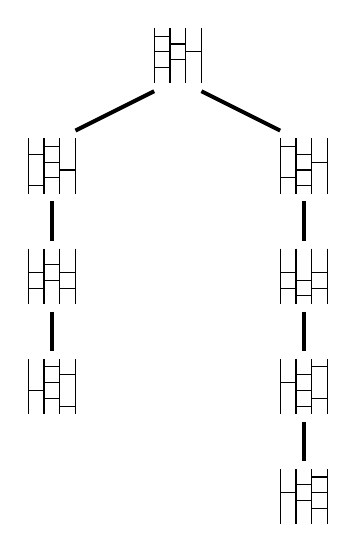
\begin{tikzpicture}
		%%L1
		\draw(5, 10) to (5, 9.3);
			\draw(5, 9.9) to (5.2, 9.9);
			\draw(5.2, 9.8) to (5.4, 9.8);
			\draw(5.4, 9.7) to (5.6, 9.7);
		\draw(5.2, 10) to (5.2, 9.3);
			\draw(5, 9.7) to (5.2, 9.7);
			\draw(5.2, 9.6) to (5.4, 9.6);
		\draw(5.4, 10) to (5.4, 9.3);
			\draw(5, 9.5) to (5.2, 9.5);
		\draw(5.6, 10) to (5.6, 9.3);
		%L2
		\draw[line width = .5mm](5, 9.2) to (4, 8.7);
		\draw[line width = .5mm](5.6, 9.2) to (6.6, 8.7);
			%%L2
			\draw(3.4, 8.6) to (3.4, 7.9);
				\draw(3.4, 8.4) to (3.6, 8.4);
				\draw(3.4, 8) to (3.6, 8);
			\draw(3.6, 8.6) to (3.6, 7.9);
				\draw(3.6, 8.5) to (3.8, 8.5);
				\draw(3.6, 8.3) to (3.8, 8.3);
				\draw(3.6, 8.1) to (3.8, 8.1);
			\draw(3.8, 8.6) to (3.8, 7.9);
				\draw(3.8, 8.2) to (4, 8.2);
			\draw(4.0, 8.6) to (4.0, 7.9);

				%%level
				\draw[line width = .5mm](3.7, 7.8) to (3.7, 7.3);
			\draw(3.4, 7.2) to (3.4, 6.5);
				\draw(3.4, 6.9) to (3.6, 6.9);
				\draw(3.4, 6.7) to (3.6, 6.7);
			\draw(3.6, 7.2) to (3.6, 6.5);
				\draw(3.6, 7) to (3.8, 7);
				\draw(3.6, 6.8) to (3.8, 6.8);
			\draw(3.8, 7.2) to (3.8, 6.5);
				\draw(3.8, 6.9) to (4, 6.9);
				\draw(3.8, 6.7) to (4, 6.7);
			\draw(4.0, 7.2) to (4.0, 6.5);

		%%L3
			\draw(6.6, 8.6) to (6.6, 7.9);
				\draw(6.6, 8.5) to (6.8, 8.5);
				\draw(6.8, 8.4) to (7, 8.4);
				\draw(7, 8.3) to (7.2, 8.3);
			\draw(6.8, 8.6) to (6.8, 7.9);
				\draw(6.8, 8.2) to (7, 8.2);
				\draw(6.8, 8) to (7, 8);
			\draw(7, 8.6) to (7, 7.9);
				\draw(6.6, 8.1) to (6.8, 8.1);
			\draw(7.2, 8.6) to (7.2, 7.9);
			
			
			\draw[line width = .5mm](6.9, 7.8) to (6.9, 7.3);

			\draw(6.6, 7.2) to (6.6, 6.5);
				\draw(6.6, 6.9) to (6.8, 6.9);
				\draw(6.6, 6.7) to (6.8, 6.7);
			\draw(6.8, 7.2) to (6.8, 6.5);
				\draw(6.8, 6.8) to (7, 6.8);
				\draw(6.8, 6.6) to (7, 6.6);
			\draw(7.0, 7.2) to (7.0, 6.5);
				\draw(7, 6.9) to (7.2, 6.9);
				\draw(7, 6.7) to (7.2, 6.7);
			\draw(7.2, 7.2) to (7.2, 6.5);

			\draw[line width = .5mm](3.7, 6.4) to (3.7, 5.9);

			\draw(3.4, 5.8) to (3.4, 5.1);
				\draw(3.4, 5.4) to (3.6, 5.4);
			\draw(3.6, 5.8) to (3.6, 5.1);
				\draw(3.6, 5.7) to (3.8, 5.7);

				\draw(3.6, 5.5) to (3.8, 5.5);
				\draw(3.6, 5.3) to (3.8, 5.3);
			\draw(3.8, 5.8) to (3.8, 5.1);
				\draw(3.8, 5.6) to (4, 5.6);
				\draw(3.8, 5.2) to (4, 5.2);
			\draw(4.0, 5.8) to (4.0, 5.1);

			\draw[line width = .5mm](6.9, 6.4) to (6.9, 5.9);

			
			\draw(6.6, 5.8) to (6.6, 5.1);
				\draw(6.6, 5.5) to (6.8, 5.5);
			\draw(6.8, 5.8) to (6.8, 5.1);
				\draw(6.8, 5.6) to (7, 5.6);

				\draw(6.8, 5.4) to (7, 5.4);
				\draw(6.8, 5.2) to (7, 5.2);
			\draw(7.0, 5.8) to (7.0, 5.1);
				\draw(7.0, 5.7) to (7.2, 5.7);
				\draw(7.0, 5.3) to (7.2, 5.3);
			\draw(7.2, 5.8) to (7.2, 5.1);

			\draw[line width = .5mm](6.9, 5) to (6.9, 4.5);

			\draw(6.6, 4.4) to (6.6, 3.7);
				\draw(6.6, 4.1) to (6.8, 4.1);
			\draw(6.8, 4.4) to (6.8, 3.7);
				\draw(6.8, 4.2) to (7, 4.2);

				\draw(6.8, 4) to (7, 4);
			\draw(7.0, 4.4) to (7.0, 3.7);
				\draw(7.0, 4.3) to (7.2, 4.3);
				\draw(7.0, 4.1) to (7.2, 4.1);
				\draw(7.0, 3.9) to (7.2, 3.9);
			\draw(7.2, 4.4) to (7.2, 3.7);



	\end{tikzpicture}
	\caption{The tree structure of $OptL\{(4,3,2,1)\}$ generated by {\sc FindAllChildren}}
	\label{Fig:TreeFAC}
\end{figure}
\pagebreak
Each $OptL\{\pi\}$ has a unique ladder which is the root of the tree generated by {\sc FindAllChildren}. This ladder 
is known as the \emph{root ladder}. Unlike every other ladder in the tree, 
the root ladder cannot be derived from a local swap operation. Thus, the root ladder 
must be created by another algorithm other than {\sc FindAllChildren}. In Chapter 3, the algorithm 
for creating the root ladder along with further information regarding the root ladder is provided. 
To see the root ladder of $OptL\{(4,5,6,3,1,2)\}$ please refer to figure Figure~\ref{fig:root}. 
In Chapter 3, section titled The Root Ladder in Detail, we discuss the details of the root ladder in relation to the Canonical Ladder Listing Problem.

%%%%%%%%%%%%%ROOT LADDER FIGURE%%%%%%%%%%%%%%%%%%%%%%%
\begin{figure}[h]


	\begin{center}
		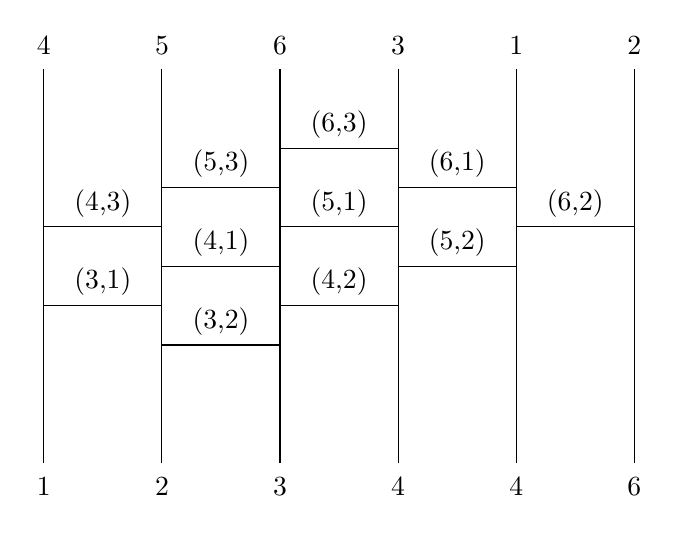
\begin{tikzpicture}
			%%draw the lines
			\draw(0, 0) to (0, 5);
				\node at (0, 5.3){4};
				\node at (0, -0.3){1};

			\draw(1.5, 0) to (1.5, 5);
				\node at (1.5, 5.3){5};
				\node at (1.5, -0.3){2};
			
			\draw(3, 0) to (3, 5);
				\node at (3, 5.3){6};
				\node at (3, -0.3){3};
			\draw(4.5, 0) to (4.5, 5);
				\node at (4.5, 5.3){3};
				\node at (4.5, -0.3){4};
			\draw(6, 0) to (6, 5);
				\node at (6, 5.3){1};
				\node at (6, -0.3){4};
			\draw(7.5, 0) to (7.5, 5);
				\node at (7.5, 5.3){2};
				\node at (7.5, -0.3){6};

			%%draw the bars
			
			%%6's route
			\draw(3, 4) to (4.5, 4);
				\node at (3.75, 4.3){(6,3)};
			\draw(4.5, 3.5) to (6, 3.5);
				\node at (5.25, 3.8){(6,1)};
			\draw(6, 3) to (7.5, 3);
				\node at (6.75, 3.3){(6,2)};
			%%5's route
			\draw(1.5, 3.5) to (3, 3.5);
				\node at (2.25, 3.8){(5,3)};
			\draw(3, 3) to (4.5, 3);
				\node at (3.75, 3.3){(5,1)};
			\draw(4.5, 2.5) to (6, 2.5);
				\node at (5.25, 2.8){(5,2)};
			%draw 4's route
			\draw(0, 3) to (1.5, 3);
				\node at (0.75, 3.3){(4,3)};
			\draw(1.5, 2.5) to (3, 2.5);
				\node at (2.25, 2.8){(4,1)};
			\draw(3, 2) to (4.5, 2);
				\node at (3.75,2.3){(4,2)};

			%%draw 3's route
			\draw(0, 2) to (1.5, 2);
				\node at (0.75, 2.3){(3,1)};
			\draw(1.5, 1.5) to (3, 1.5);
				\node at (2.25, 1.8){(3,2)};
		\end{tikzpicture}

	\end{center}





	\caption{The root ladder for $OptL\{(4,5,6,3,1,2)\}$. Notice how 
	no bar associated with a lesser element is above bars associated with a greater element.
	Therefore, the clean level of this ladder is $1$, thus making it the root ladder.} 
	\label{fig:root}

\end{figure}





%%Root ladder subsection




%%DONE Appendix SECTION

In concluding the section on the enumeration problem, we have analyzed the original paper along with 
making additions to the algorithm {\sc FindAllChildren} by providing four essential algorithms 
for the completion of {\sc FindAllChildren}. The algorithms are Algorithm~\ref{Alg:RootLadder}, Algorithm~\ref{Alg:RightSwap},
Algorithm~\ref{Alg:LeftSwap} and Algorithm~\ref{Alg:ShiftSubLadder} which can be found in the Appendix. In concert, these five algorithms solve the enumeration 
problem which lists $OptL\{\pi\}$ in $O(1)$ time per ladder. 

